\chapter{Hasil dan Pembahasan}

%% VERSI BAHASA INDONESIA. Konvensi peristilahan dijelaskan pada kepala chapter-1.tex.
%% \crosscheck{...} menandai nilai yang wajib diverifikasi ulang terhadap proses FINAL
%% sebelum penyerahan. Seluruh angka di bawah adalah nilai eksperimen saat ini.

Bab ini pertama-tama merangkum sistem yang dihasilkan. Bab ini kemudian melaporkan hasil
dari setiap tingkat evaluasi yang dijelaskan pada Bab~III, yaitu kualitas pembangunan graf,
keselarasan panduan klinis dan ablasi \emph{observation gate}, validasi terhadap \emph{gold
standard} manual, deteksi keamanan, \emph{faithfulness} ringkasan, dan telaah klinisi. Bab ini
ditutup dengan perbandingan terhadap penelitian terdahulu serta pembahasan. Seluruh tingkat
evaluasi bersifat otomatis kecuali telaah klinisi, yang cakupannya terbatas sebagaimana
diuraikan pada Subbab~\ref{sec:limitations}.

Setiap subbab menjawab satu tujuan penelitian spesifik dari Subbab~1.3.
Tabel~\ref{tab:ro-map} menyatakan pemetaannya secara eksplisit.

\begin{table}[h]
\centering
\caption{Pemetaan tujuan penelitian terhadap subbab yang menjawabnya.}
\label{tab:ro-map}
\begin{tabular}{@{}p{96mm}p{46mm}@{}}
\hline
\textbf{Tujuan penelitian} & \textbf{Dijawab pada} \\
\hline
RO1 -- Alur FHIR-native, \emph{knowledge graph}, jembatan konsep, dan evaluasi menyeluruh
    & Subbab \ref{sec:sys-impl}, \ref{sec:kg-results}, \ref{sec:gold},
      \ref{sec:safety-detection}, \ref{sec:clinician} \\
RO2 -- \emph{Observation gate} dan ablasi keselarasan
    & Subbab \ref{sec:ablation} \\
RO3 -- \emph{Grounded briefing} dan \emph{faithfulness}-nya
    & Subbab \ref{sec:faithfulness} \\
\hline
\end{tabular}
\end{table}

\section{Implementasi Sistem}
\label{sec:sys-impl}

Rancangan pada Bab~III direalisasikan sebagai sehimpunan program Python yang bekerja di atas
\emph{knowledge graph} Neo4j. Komponen utamanya adalah

\begin{itemize}
    \item sebuah \textbf{\emph{loader} FHIR ke Neo4j} yang memetakan setiap \emph{resource}
    FHIR menjadi simpul, setiap rujukan menjadi relasi yang tipenya diambil dari nama elemen
    asalnya (\texttt{Observation.subject} menghasilkan sisi \texttt{SUBJECT}, bukan sisi
    generik), dan setiap kode terminologi
    menjadi simpul \texttt{:Code} bersama, dengan observasi bernilai jamak dimekarkan menjadi
    simpul komponen dan \emph{allow-list} observasi diterapkan; seluruh penulisan bersifat idempoten
    (\texttt{MERGE}) sehingga pemuatan ulang aman dilakukan;
    \item sebuah \textbf{jembatan terminologi} yang mengekspor kode EHR dari graf dan
    memetakannya ke konsep UMLS melalui \emph{linker} tiga-lintasan (alias persis,
    pembangkitan kandidat, lalu penautan berbasis NLP) sehingga menghasilkan tulang
    punggung \texttt{SAME\_CONCEPT};
    \item \textbf{lapisan panduan klinis dan literatur} yang menyimpan rekomendasi hasil kurasi manual dari panduan klinis dan
    hasil ekstraksi NLP dari korpus literatur, kemudian dihubungkan ke simpul konsep bersama;
    \item sebuah \textbf{lapisan kueri rekomendasi} yang termasuk di dalamnya rekomendasi yang dapat diberlakukan,
    \emph{observation gate}, keamanan kontraindikasi, dan pemeringkatan literatur dengan PMI; serta
    \item sebuah \textbf{alur pembuatan \emph{grounded briefing}} dengan cara menelusuri fakta pendukung
    keputusan secara deterministik dan meminta model bahasa besar merumuskan ringkasannya, disusul
    pemeriksaan \emph{faithfulness} otomatis.
\end{itemize}

Tabel~\ref{tab:modules} mencantumkan modul implementasi beserta fungsinya. Sistem
diimplementasikan dalam Python, dengan Cypher untuk tahap pembangunan graf, pada basis data
Neo4j; \emph{knowledge graph} dibangun satu kali lalu dikueri per pasien.

\begin{table}[h]
\centering
\caption{Modul implementasi beserta fungsinya.}
\label{tab:modules}
\begin{tabular}{@{}p{42mm}p{100mm}@{}}
\hline
\textbf{Modul} & \textbf{Fungsi} \\
\hline
\emph{Loader}\newline{\scriptsize \texttt{loader.py}} & Memuat \emph{bundle} FHIR R4 ke Neo4j (simpul, sisi, simpul \texttt{:Code} bersama) \\
Ekspor kode\newline{\scriptsize \texttt{graph\_export\_ehr\_codes.py}} & Mengekspor kode EHR terdeduplikasi dari graf untuk dijembatani \\
Jembatan UMLS\newline{\scriptsize \texttt{snomed\_umls\_bridge.py}} & Memetakan kode EHR ke CUI UMLS (\emph{linker} tiga-lintasan) \\
Lapisan konsep\newline{\scriptsize \texttt{ehr\_concept\_kg.cypher}} & Membuat konsep dan sisi \texttt{SAME\_CONCEPT} ke simpul \texttt{:Code} \\
Lapisan panduan\newline{\scriptsize \texttt{guideline\_kg.cypher}} & Memuat rekomendasi, sisi turunan COR, dan sitasi \\
Lapisan literatur\newline{\scriptsize \texttt{literature\_kg.cypher}} & Memuat abstrak, sebutan entitas, dan sisi kemunculan bersama PMI \\
\emph{Observation gate}\newline{\scriptsize \texttt{obs\_gate.py}} & Memutuskan rekomendasi bergantung-observasi dari fitur graf \\
Kronisitas NSAID\newline{\scriptsize \texttt{nsaid\_csv.py}} & Menghitung status NSAID kronis dari durasi periode penggunaan dari CSV \\
Rekomendasi/evaluasi\newline{\scriptsize \texttt{crs\_eval.py}, \texttt{eval\_by\_class.py}} & Himpunan kueri, keamanan, dan literatur; penilaian keselarasan \\
Standar rujukan (\emph{oracle})\newline{\scriptsize \texttt{silver\_oracle.py}} & Label independen-CRS yang dibaca dari \emph{bundle} FHIR mentah \\
\emph{Grounded briefing}\newline{\scriptsize \texttt{crs\_briefing.py}} & Penelusuran deterministik + perumusan oleh LLM \\
Pemeriksa \emph{faithfulness}\newline{\scriptsize \texttt{faithfulness\_check.py}} & Memverifikasi ringkasan terhadap fakta hasil penelusuran \\
\hline
\end{tabular}
\end{table}

Tiap modul diberi nama bersebelahan dengan nama berkas sumbernya. Lampiran~\ref{app:modules}
mencantumkan skrip pendukungnya dan memuat ulang tiga \emph{listing} yang membawa
keputusan rancangan yang menjadi tumpuan teks ini: \texttt{MERGE} idempoten pada
\emph{loader}, predikat \emph{observation gate}, dan \emph{prompt} \emph{briefing}.

Gambar~\ref{fig:architecture} menempatkan modul-modul pada Tabel~\ref{tab:modules} ke dalam sistem
yang terancang. Model bahasa berada di ujung tahapan dan hanya menerima apa yang telah
dirakit penelusuran deterministik. Standar rujukannya dihitung dari rekam medis mentah, bukan dari \emph{knowledge graph} yang
terbentuk.

\begin{figure}[htbp]
\centering
\resizebox{\textwidth}{!}{%
\begin{tikzpicture}[
    node distance = 9mm and 3mm,
    box/.style   = {rectangle, rounded corners=2pt, draw, text width=22mm,
                    align=center, minimum height=11mm, font=\scriptsize},
    src/.style   = {box, fill=black!5},
    store/.style = {rectangle, rounded corners=2pt, draw, very thick, fill=black!12,
                    text width=129.5mm, align=center, minimum height=12mm, font=\scriptsize},
    pay/.style   = {rectangle, rounded corners=2pt, draw, dashed,
                    text width=129.5mm, align=center, minimum height=9mm, font=\scriptsize},
    ev/.style    = {box, fill=black!8},
    fn/.style    = {font=\tiny},
    band/.style  = {font=\scriptsize\itshape, inner sep=0pt},
    ar/.style    = {-latex, thick},
    raw/.style   = {-latex, dashed}
]
\node[src] (s1) {\emph{Bundle} FHIR R4 Synthea\\[1pt]\emph{5.490 pasien}};
\node[src, right=of s1] (s2) {Ekspor CSV Synthea\\[1pt]\emph{tanggal mulai/berhenti}};
\node[src, right=of s2] (s3) {UMLS \emph{Metathesaurus}};
\node[src, right=of s3] (s4) {Abstrak PubMed\\[1pt]\emph{4.801, berbenih panduan klinis}};
\node[src, right=of s4] (s5) {Panduan CCD AHA/ACC 2023};

\node[box, below=of s1] (b1) {Lapisan EHR\\[1pt]{\fn\texttt{loader.py}}};
\node[box, right=of b1] (b2) {Ekspor kode\\[1pt]{\fn\texttt{graph\_export\_}\\\texttt{ehr\_codes.py}}};
\node[box, right=of b2] (b3) {Jembatan UMLS\\[1pt]{\fn\texttt{snomed\_umls\_}\\\texttt{bridge.py}}};
\node[box, right=of b3] (b4) {Lapisan konsep dan literatur\\[1pt]{\fn\texttt{ehr\_concept\_kg}\\\texttt{literature\_kg}\\(\texttt{.cypher})}};
\node[box, right=of b4] (b5) {Lapisan panduan klinis\\[1pt]{\fn\texttt{guideline\_kg}\\\texttt{.cypher}}};

\node[store, below=9mm of b3] (store)
    {\textbf{\texttt{sihdfhir}} (Neo4j)\\[1pt]
     lapisan EHR $\cdot$ konsep $\cdot$ panduan klinis $\cdot$ literatur\\[1pt]
     \emph{1.804.379 simpul, 8.796.425 relasi}};

\node[box, below=9mm of store.south west, anchor=north west] (v1)
    {Himpunan berlaku\\[1pt]\emph{gerbang CCD, lalu AND/OR}};
\node[box, right=of v1] (v2) {\emph{Observation gate}\\[1pt]{\fn\texttt{obs\_gate.py}}};
\node[box, right=of v2] (v3) {Tanda keamanan\\[1pt]\emph{kontraindikasi}};
\node[box, right=of v3] (v4) {Dukungan literatur\\[1pt]\emph{pemeringkatan PMI}};
\node[box, right=of v4] (v5) {Kronisitas NSAID\\[1pt]{\fn\texttt{nsaid\_csv.py}}};

\node[pay, below=9mm of v3] (facts)
    {\emph{Facts payload}\\[1pt]\emph{tiap butir membawa pengenal rekomendasi, COR, dan PMID}};

\node[box, below=9mm of facts.south west, anchor=north west] (p1)
    {Model bahasa\\[1pt]\emph{hanya merumuskan}};
\node[box, right=of p1] (p2) {\emph{Briefing}\\[1pt]\emph{utama + rincian}};
\node[box, right=of p2] (p3) {Pemeriksaan \emph{faithfulness}\\[1pt]{\fn\texttt{faithfulness\_}\\\texttt{check.py}}};

\node[ev, below=9mm of p1] (e1)
    {Standar rujukan\\[1pt]{\fn\texttt{silver\_oracle.py}}};
\node[ev, right=of e1] (e2)
    {Keselarasan dan ablasi\\[1pt]{\fn\texttt{crs\_eval.py}\\\texttt{eval\_by\_class.py}}};

\node[band, anchor=south west] at ([yshift=1mm]s1.north west) {Sumber};
\node[band, anchor=south west] at ([yshift=1mm]b1.north west) {Pembangunan, sekali jalan};
\node[band, anchor=south west] at ([yshift=1mm]v1.north west) {Per pasien};
\node[band, anchor=south west] at ([yshift=1mm]e1.north west) {Evaluasi};

% sources into the build
\draw[ar] (s1) -- (b1);
\draw[ar] (s3) -- (b3);
\draw[ar] (s4) -- (b3);
\draw[ar] (s5) -- (b5);

% build writes the store; the code export reads it back
\draw[ar] (b1) -- (store.north -| b1);
\draw[ar] (store.north -| b2) -- (b2);
\draw[ar] (b2) -- (b3);
\draw[ar] (b3) -- (b4);
\draw[ar] (b4) -- (store.north -| b4);
\draw[ar] (b5) -- (store.north -| b5);

% every per-patient query reads the same store
\draw[ar] (store.south -| v1) -- (v1);
\draw[ar] (store.south -| v2) -- (v2);
\draw[ar] (store.south -| v3) -- (v3);
\draw[ar] (store.south -| v4) -- (v4);
\draw[ar] (store.south -| v5) -- (v5);

% retrieval assembles the payload; the model only phrases it
\draw[ar] (v1) -- (facts.north -| v1);
\draw[ar] (v2) -- (facts.north -| v2);
\draw[ar] (v3) -- (facts.north -| v3);
\draw[ar] (v4) -- (facts.north -| v4);
\draw[ar] (v5) -- (facts.north -| v5);
\draw[ar] (facts.south -| p1) -- (p1);
\draw[ar] (p1) -- (p2);
\draw[ar] (p2) -- (p3);
\draw[ar] (facts.south -| p3) -- (p3);

% the evaluator queries the store; the reference standard never does
\coordinate (lm1) at ([xshift=-8mm]s1.west);
\coordinate (lm2) at ([xshift=-13mm]s1.west);
\draw[raw] (s1.west) -- (lm1) |- ([yshift=2mm]e1.west);
\draw[raw] (s2.north) -- ++(0,7mm) -| (lm2) |- ([yshift=-2mm]e1.west);
\draw[ar] (e1) -- (e2);
\draw[ar] (store.east) -- ++(8mm,0) |- (e2.east);
\end{tikzpicture}}
\caption{Arsitektur sistem. Pembangunan berjalan sekali dan menuliskannya di satu
tempat penyimpanan; ekspor kode membaca kembali penyimpanan tersebut dan karena itulah jembatan UMLS
menautkan persis semesta kode yang benar-benar dimiliki graf. Setiap kueri per pasien
kemudian membaca graf yang sama, sedangkan model bahasa berada di ujung rantai tanpa adanya jalan
kembali ke graf itu. Dua panah putus-putus merupakan sifat ketaksirkularannya: standar
rujukan dihitung dari rekam medis mentah---\emph{bundle}-nya serta ekspor CSV untuk durasi
pengobatan yang dibuang FHIR---sementara penilainya mengueri dari penyimpanan sehingga kedua sisi
tidak pernah berbagi penurunan. Validasi standar rujukan tersebut terhadap 30 pasien yang
dilabeli manual diuraikan pada Subbab~\ref{sec:gold} dan tidak digambarkan di sini.}
\label{fig:architecture}
\end{figure}

\section{Hasil Pembangunan \emph{Knowledge Graph}}
\label{sec:kg-results}

Graf yang terbangun (basis data \texttt{sihdfhir}) memuat 1.804.379 simpul dan
8.796.425 relasi. Tabel~\ref{tab:graph-scale} merangkum graf tersebut menurut
tiga dimensi struktural yang ditetapkan pada Subbab~\ref{sec:structural}---\emph{richness},
\emph{width}, dan \emph{depth}---mengikuti kerangka ukuran struktural pada evaluasi ontologi
\cite{gangemi2006}, dengan \emph{richness} mengikuti OntoQA \cite{tartir2005} dan
\emph{width} bersesuaian dengan dimensi \emph{completeness} pada mutu \emph{knowledge graph}
\cite{issa2021}. Sebagaimana dicatat di subbab tersebut, \emph{depth} didefinisikan ulang untuk graf
properti sebagai panjang lintasan inferensi, bukan kedalaman hierarki \texttt{is-a}.
Tabel~\ref{tab:graph-counts} mencantumkan populasi simpul utamanya.

\begin{table}[h]
\centering
\caption{Metrik mutu intrinsik graf. Derajat-masuk simpul pusat adalah banyaknya simpul \emph{resource} yang menunjuk ke satu
simpul \texttt{:Code} sehingga angka itu mengukur seberapa luas sebuah kode dipakai ulang. Angka tersebut dihitung
atas 1.321 kode yang berasal dari terminologi klinis (SNOMED~CT, RxNorm, LOINC, CVX).}
\label{tab:graph-scale}
\begin{tabular}{@{}p{24mm}p{68mm}p{46mm}@{}}
\hline
\textbf{Dimensi} & \textbf{Metrik} & \textbf{Nilai} \\
\hline
\emph{Richness} & Label simpul berbeda            & 25 \\
                & Tipe relasi berbeda             & 51 \\
                & Sistem kode berbeda             & 26 \\
                & Sumber bukti yang disatukan (EHR, panduan klinis, literatur) & 3 \\
\emph{Width}    & Simpul/relasi                 & 1.804.379/8.796.425 \\
                & Pasien                          & 5.490 \\
                & Rerata kondisi per pasien       & 23,9 \\
                & Konsep UMLS (EHR/literatur)   & 514/4.161 \\
\emph{Depth}    & Lintasan inferensi kanonis & 5 lompatan, 6 simpul \\
                & Derajat-masuk simpul pusat kode klinis (rerata/maks) & 1.578/108.617 \\
\hline
\end{tabular}
\end{table}

\begin{table}[h]
\centering
\caption{Populasi simpul utama dalam \emph{knowledge graph}.}
\label{tab:graph-counts}
\begin{tabular}{lr@{\hskip 2cm}lr}
\hline
\textbf{Tipe simpul} & \textbf{Cacah} & \textbf{Tipe simpul} & \textbf{Cacah} \\
\hline
Patient          & 5.490   & Medication      & 70.486  \\
Condition        & 131.465 & Component       & 105.166 \\
Procedure        & 593.922 & Code (bersama)  & 1.395   \\
Observation      & 242.217 & Concept (UMLS)  & 4.556   \\
MedicationRequest& 193.019 & Recommendation  & 81      \\
Abstract         & 4.801   & & \\
\hline
\end{tabular}
\end{table}

Jumlah simpul \texttt{:Patient} sebesar 5.490 sama dengan jumlah pasien yang dilaporkan Synthea dari hasil
pembangkitan kedua proses (Subbab~\ref{sec:cohort}), yang menegaskan bahwa pemuatan
idempoten tidak membuang maupun menggandakan satu pun rekam medis pasien.

Angka-angka ini memperlihatkan graf yang benar-benar heterogen (25 label, 51 tipe relasi, 26
sistem kode), luas (5.490 pasien dengan rerata 23,9
kondisi pada setiap pasien), dan terhubung dengan tiga sumber bukti melalui simpul pusat
\texttt{:Code} bersama. Setiap kode terminologi klinis dirujuk oleh rata-rata
1.578 \emph{resource}---bukti bahwa rancangan jangkar bersama mengurangi
keberulangan terminologi alih-alih menggandakannya.

\section{Keselarasan Panduan Klinis dan Ablasi \emph{Observation Gate}}
\label{sec:ablation}

Keselarasan panduan klinis diukur terhadap \emph{silver standard} yang independen dari sistem
rekomendasi atas kohort 876 pasien yang dapat dievaluasi gerbang.
Tabel~\ref{tab:ablation} melaporkan eksperimen utamanya: sistem dengan dan tanpa
\emph{observation gate}.

\begin{table}[h]
\centering
\caption{Ablasi \emph{observation gate} (keselarasan panduan klinis terhadap \emph{silver standard},
rerata makro).}
\label{tab:ablation}
\begin{tabular}{lccc}
\hline
\textbf{Konfigurasi} & \textbf{Presisi} & \textbf{\emph{Recall}} & \textbf{$F_1$} \\
\hline
\emph{Baseline} (gerbang + AND, tanpa \emph{observation gate}) & 0,612 & 0,948 & 0,743 \\
\textbf{+ \emph{observation gate}} & \textbf{0,684} & \textbf{0,994} & \textbf{0,810} \\
\hline
\end{tabular}
\end{table}

\begin{figure}[htbp]
\centering
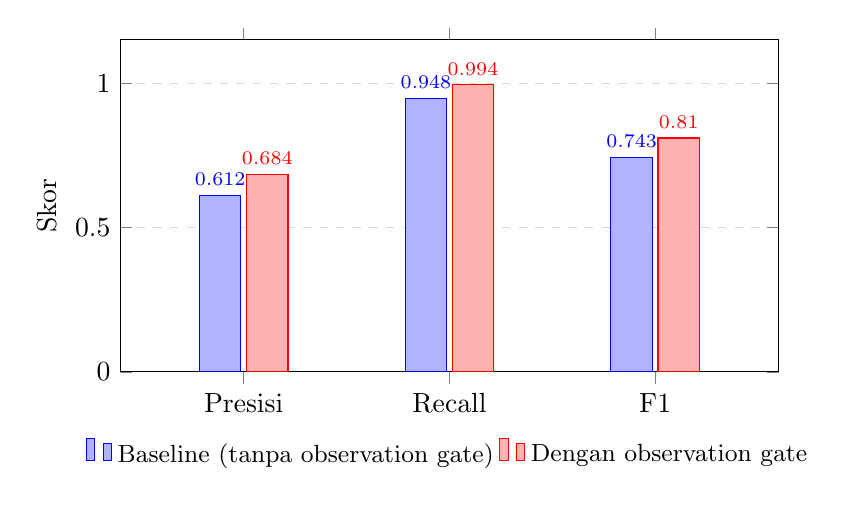
\begin{tikzpicture}
\begin{axis}[
    ybar,
    width=0.82\textwidth,
    height=58mm,
    bar width=15pt,
    ymin=0, ymax=1.15,
    ylabel={Skor},
    symbolic x coords={Presisi, Recall, F1},
    xtick=data,
    nodes near coords,
    nodes near coords style={font=\scriptsize, /pgf/number format/fixed,
                             /pgf/number format/precision=3},
    legend style={at={(0.5,-0.18)}, anchor=north, legend columns=2, font=\small,
                  draw=none},
    enlarge x limits=0.3,
    ymajorgrids=true,
    grid style={dashed, gray!30},
]
\addplot coordinates {(Presisi,0.612) (Recall,0.948) (F1,0.743)};
\addplot coordinates {(Presisi,0.684) (Recall,0.994) (F1,0.810)};
\legend{Baseline (tanpa observation gate), Dengan observation gate}
\end{axis}
\end{tikzpicture}
\caption{Ablasi \emph{observation gate}. Penggerbangan menaikkan presisi tanpa mengorbankan
\emph{recall} sehingga menghasilkan kenaikan $F_1$ neto.}
\label{fig:ablation}
\end{figure}

Sebagaimana diperlihatkan Gambar~\ref{fig:ablation}, \emph{observation gate} menaikkan $F_1$
sebesar $+0{,}067$ (dari 0,743 menjadi 0,810), yang disebabkan oleh kenaikan
presisi (rekomendasi berprasyarat numerik tidak lagi muncul bagi setiap pasien CCD) dengan
\emph{recall} yang praktis tidak berubah. Karena kedua konfigurasi berbagi \emph{baseline}
yang sama, ablasi ini mengisolasi kontribusi \emph{observation gate} itu sendiri. Ablasi ini tidak mengisolasi kontribusi wadah datanya. Pertanyaan apakah perolehan tersebut memang
menuntut FHIR merupakan pertanyaan yang terpisah dan diuji tersendiri pada
Subbab~\ref{sec:csv-gating}.

\subsection{Dari mana kenaikan tersebut berasal}
\label{sec:ablation-class}
Perlu dipahami angka pada Tabel~\ref{tab:ablation} dan Gambar~\ref{fig:ablation} merupakan angka rata-rata dari 68 rekomendasi sehingga sumber kenaikan angka tersebut perlu dilihat berdasarkan masing-masing rekomendasi.
Subbab~\ref{sec:disc-class} memilah 68 rekomendasi nonkontraindikasi menurut cara
masing-masing mempersempit kohort dan hanya 15 rekomendasi yang membawa prasyarat numerik
yang dinilai berbeda ketika penggerbangan dinyalakan. Ke-53 rekomendasi sisanya memberi
jawaban yang sama pada kedua keadaan sehingga mereka menurunkan rerata tanpa menyumbang
apa pun pada perubahan yang hendak diperlihatkan rerata itu. Tabel~\ref{tab:ablation-class} melaporkan keselarasan secara terpisah untuk
setiap kelas pada kedua lengan.

\begin{table}[h]
\centering
\caption{Keselarasan menurut kelas pembeda pada kedua lengan ablasi, rerata mikro dari kohort
876 pasien. Kelasnya mengikuti Subbab~\ref{sec:disc-class}: rekomendasi
\emph{universal} sama sekali tidak membawa mekanisme untuk mempersempit kohort,
\emph{concept-matched} mensyaratkan target kondisi lanjutan, \emph{value-gated} mensyaratkan
predikat numerik atas sebuah observasi, dan \emph{both} mensyaratkan keduanya sekaligus. Kedua
kelas yang tidak tergerbang identik pada kedua lengan hingga cacah satuannya; seluruh efek
ablasi hanya berdampak pada 15 rekomendasi yang tergerbang.}
\label{tab:ablation-class}
\footnotesize
\setlength{\tabcolsep}{4pt}
\begin{tabular}{lr|ccc|ccc}
\hline
& & \multicolumn{3}{c|}{\textbf{\emph{Baseline} (tanpa gerbang)}}
  & \multicolumn{3}{c}{\textbf{Dengan \emph{observation gate}}} \\
\textbf{Kelas} & \textbf{rek.} & \textbf{P} & \textbf{R} & \textbf{$F_1$}
                               & \textbf{P} & \textbf{R} & \textbf{$F_1$} \\
\hline
Universal        & 38 & 0,666 & 1,000 & 0,799 & 0,666 & 1,000 & 0,799 \\
Tercocok-konsep  & 15 & 0,676 & 0,915 & 0,777 & 0,676 & 0,915 & 0,777 \\
Tergerbang-nilai & \phantom{0}5 & 0,194 & 1,000 & 0,325
                                & \textbf{1,000} & \textbf{1,000} & \textbf{1,000} \\
Keduanya         & 10 & 0,038 & 0,006 & 0,011
                                & \textbf{1,000} & \textbf{1,000} & \textbf{1,000} \\
\hline
\textbf{Semua}   & 68 & 0,613 & 0,945 & 0,743 & 0,685 & 0,993 & 0,811 \\
\hline
\end{tabular}
\end{table}

Didapatkan empat hasil pembacaan hasil dari Tabel~\ref{tab:ablation-class}.

Pertama, kedua kelas yang tidak tergerbang \emph{identik} pada kedua lengan---bukan hanya
hampir sama, melainkan sama hingga ke cacah satuan \emph{true positive}, \emph{false positive},
dan \emph{false negative} ($22.158/11.130/0$ untuk kelas universal, $2.018/969/188$ untuk
kelas dengan konsep yang cocok). Oleh karena itu, 53 dari 68 rekomendasi tidak tersentuh dan
seluruh selisih $F_1$ yang dilaporkan berasal dari 15 rekomendasi sisanya. Hal ini merupakan
prediksi yang dapat difalsifikasi dari klasifikasi pada Subbab~\ref{sec:disc-class} dan
prediksi tersebut terbukti persis.

Kedua, kedua kelas yang tergerbang memperoleh manfaat dengan cara yang berlawanan. Bagi kelima rekomendasi
\emph{tergerbang-nilai}, penggerbangan merupakan mekanisme \emph{presisi}: tanpa
penggerbangan, rekomendasi tersebut muncul bagi setiap anggota kohort (849 \emph{true positive}
berbanding 3.531 \emph{false positive}, $P = 0{,}194$) dan dengan penggerbangan, rekomendasi
tersebut hanya muncul bila nilai terukur memenuhi predikatnya ($P = 1{,}000$), sementara
\emph{recall}-nya memang sudah sempurna. Bagi kelas \emph{keduanya}, penggerbangan justru sangat dominan sebagai mekanisme
\emph{recall}. Pada lengan \emph{baseline}, kesepuluh rekomendasi tersebut nyaris tidak
pernah muncul sama sekali (8 \emph{true positive} berbanding 1.263 \emph{false negative}, $R
= 0{,}006$) karena target kondisinya yang terkodekan saja jarang cocok. Predikat observasi
itulah yang sesungguhnya mengenali pasien yang dikenai rekomendasi tersebut.
Menggambarkan ablasi semata-mata sebagai perbaikan presisi menjadi keliru bagi dua pertiga rekomendasi yang terpengaruh.

Ketiga, kedua kelas yang tergerbang mencapai $P = R = 1{,}000$ setelah penggerbangan
dinyalakan. Nilai sempurna itu mengatakan sesuatu tentang urusan teknisnya, bukan tentang
seberapa sulit penilaian klinisnya. \emph{Observation gate} dan standar rujukan menerapkan ambang panduan klinis yang sama,
misalnya fraksi ejeksi 40\% atau kurang. Namun, keduanya membaca nilai pasien dari tempat
yang berbeda. Gerbang membacanya dari graf, sedangkan standar rujukan membacanya dari
\emph{bundle} FHIR mentah. Karena itu, kesepakatan pada setiap pasien
menunjukkan bahwa \emph{loader} membawa nilai-nilai tersebut tanpa mengubahnya. Hal itu tidak
menunjukkan bahwa ambangnya benar secara klinis sebab kedua sisi memang diberi ambang yang
sama sejak awal. Subbab~\ref{sec:shared-predicate} memastikan bahwa keduanya memang fungsi yang
sama, lalu mengukur seberapa besar bagian angka keselarasan yang bertumpu pada hal tersebut.

Keempat, lima dari sepuluh rekomendasi kelas \emph{both} bersifat \emph{tidak aktif}.
\texttt{TP:2}, \texttt{TP:3:1}, \texttt{TP:3:2}, \texttt{TP:4}, dan \texttt{TP:5} mencatat nol
\emph{true positive}, nol \emph{false positive}, dan nol \emph{false negative} pada \emph{kedua}
lengan sehingga tidak menyumbang apa pun pada kolom mana pun. Kelimanya digerbangi oleh satu
predikat yang sama---merokok aktif setiap hari---yang tidak dipenuhi satu pun pasien dalam
kohort: dari 876 pasien, 390 tercatat tidak pernah merokok,
237 sebagai mantan perokok, 249 sama sekali tidak membawa observasi
status merokok, dan 0 merupakan perokok aktif. Karena itu, baris \emph{both}
sepenuhnya ditentukan oleh lima rekomendasi yang aktif dan cacah yang dikutip di atas bagian dari
kelima rekomendasi tersebut, bukan bagian dari sepuluh lainnya. \texttt{LIPID:9} tidak aktif karena alasan
sejenis---tidak ada pasien kohort yang memenuhi konjungsinya---sehingga gerbang yang
diperolehnya ketika trigliserida dimuat tidak pernah terpakai.

Hal ini berlaku lebih luas daripada hanya sebatas pada kelas-kelas yang tergerbang. Sebanyak 22 dari
73 pengenal rekomendasi dalam berkas label rujukan tidak memiliki satu pun hasil
positif di seluruh kohort. Hal tersebut merupakan sifat dari penggunaan populasi sintetis, bukan akibat pengodeannya:
rekomendasinya terkodekan dengan benar dan akan menyala bila pasien yang relevan hadir. Namun, hal
tersebut tetap membatasi apa yang dapat ditunjukkan angka keselarasan ini dan kohort nyata akan
mengaktifkan subhimpunan yang berbeda serta mungkin lebih besar. Subbab~\ref{sec:module-yield} menunjukkan penyebab utamanya. Sebanyak 249 dari 876 pasien,
sekitar 28\%, berasal dari proses Synthea yang diperkaya penyakit. Rekam medis mereka hanya
membawa satu diagnosis penyakit jantung iskemik, satu temuan pencitraan jantung yang
abnormal, dan kadang riwayat \emph{bypass}, tanpa komorbiditas dan, selain fraksi ejeksi,
tanpa observasi apa pun.

Ada satu pilihan perataan (\emph{averaging}) yang berlaku di seluruh tabel ini. Angka-angkanya dirata-ratakan secara \emph{mikro}: seluruh
positif benar, positif salah, dan negatif salah pada kohort dijumlahkan lebih dahulu, lalu
rasionya dihitung sekali saja di akhir.

Pilihan yang lain, perataan \emph{makro}, menilai tiap pasien sendiri-sendiri lalu
merata-ratakan nilai itu. Cara tersebut tidak dapat dipakai di sini. Penyebabnya, seorang pasien dapat sama sekali tidak tersentuh oleh suatu kelas. Bagi pasien
itu, tidak ada yang dapat dijawab benar oleh sistem dan tidak ada pula yang dapat dijawab
salah sehingga ketiga cacahnya nol. Presisi, \emph{recall}, dan $F_1$-nya lalu ditetapkan
nol, bukan dibiarkan kosong. Nol itu masuk ke rerata seolah-olah
sistem gagal menangani pasien tersebut. Makin jarang suatu kelas, makin banyak pasien semacam
itu, dan makin turun pula angka makronya. Pada akhirnya, angka tersebut mengukur seberapa umum kelas itu, bukan seberapa baik sistem menanganinya.

Kelas tergerbang-nilai memperlihatkan hal ini pada ukuran penuhnya: makro $F_1 = 0{,}600$
berbanding nilai mikro $1{,}000$. Keduanya tidak saling bertentangan. Karena pada kelas itu
tidak ada satu pun positif salah maupun negatif salah, tiap pasien bernilai tepat satu atau
tepat nol sehingga angka makronya tidak lain adalah porsi kohort yang sama sekali memiliki
rekomendasi tergerbang-nilai---526 dari 876. Setiap pasien yang memang dikenai kelas tersebut
dinilai dengan sempurna. Itulah sebabnya seluruh angka per kelas yang dilaporkan di sini
dirata-ratakan secara mikro.

\subsection{Bagian mana yang dinilai secara independen}
\label{sec:shared-predicate}
Subbab~\ref{sec:oracle} memilah ketakbergantungan standar rujukan menjadi dua tingkatan. Subbab
ini melaporkan akibatnya terhadap angka yang dilaporkan.

Bagi 15 rekomendasi tergerbang-observasi, predikat sistem dan aturan standar rujukan merupakan
fungsi yang sama. Hal itu diperiksa secara empiris, bukan sekadar dibaca dari kodenya: kedua
sisi dievaluasi atas 876 vektor ciri kohort yang sesungguhnya dan atas 200.000 vektor sintetis
yang diarahkan ke tiap ambang yang diujinya, termasuk nilai yang hilang, dan tidak satu pun
dari 200.876 perbandingan itu berbeda. Karena itu, presisi dan \emph{recall} sebesar $1{,}000$
pada kedua kelas tergerbang tidak dapat dibaca sebagai penilaian atas ketepatan aturannya.

Tabel~\ref{tab:shared-predicate} memisahkan keduanya.

\begin{table}[h]
\centering
\caption{Keselarasan panduan klinis dipilah menurut tingkatan ketakbergantungan standar
rujukannya, dirata-ratakan secara mikro pada kohort 876 pasien.}
\label{tab:shared-predicate}
\begin{tabular}{lrcccrrr}
\hline
\textbf{Bagian} & \textbf{rek.} & \textbf{Presisi} & \textbf{\emph{Recall}} & \textbf{$F_1$} &
\textbf{tp} & \textbf{fp} & \textbf{fn} \\
\hline
Seluruhnya            & 68 & 0,685 & 0,993 & 0,811 & 26.296 & 12.099 & 188 \\
Predikat bersama      & 15 & 1,000 & 1,000 & 1,000 & 2.120 & 0 & 0 \\
Logika tak bergantung & 53 & 0,666 & 0,992 & 0,797 & 24.176 & 12.099 & 188 \\
\hline
\end{tabular}
\end{table}

Bagian yang dinilai penilai yang benar-benar tidak bergantung mencakup 53 dari 68 rekomendasi
dan mencatat presisi $0{,}666$ serta $F_1$ $0{,}797$. Menyingkirkan kelima belas rekomendasi
berpredikat bersama karenanya menurunkan presisi sebesar $0{,}018$ dan $F_1$ sebesar $0{,}013$;
sebanyak $8{,}1\%$ dari seluruh \emph{true positive} berasal dari bagian berpredikat bersama
tersebut. Dengan kata lain, angka utama tidak ditopang oleh bagian yang berpredikat bersama
dan kesimpulan mengenai keselarasan tetap berlaku bila bagian itu dihapus seluruhnya.

Ablasinya berbeda halnya dan hal itu perlu dinyatakan terus terang. Hanya kelas
tergerbang-nilai dan kelas keduanya yang berubah di antara kedua lengan ablasi dan keduanya
justru merupakan kelima belas rekomendasi berpredikat bersama itu. Seluruh perolehan ablasi
karenanya terukur pada rekomendasi yang standar rujukannya menerapkan aturan yang sama dengan
sistemnya. Perolehan itu tetap merupakan perubahan nyata pada perilaku sistem. Tanpa gerbang,
rekomendasi berprasyarat numerik muncul bagi pasien yang tidak memenuhi prasyarat yang
dinyatakan panduan klinis dan hal itu tetap merupakan cacat, siapa pun penilainya. Meski
begitu, perolehan itu mengukur kesetiaan implementasi, bukan keabsahan klinis. Standar rujukannya merupakan
penilai yang tidak bergantung atas nilai yang disuapkan ke aturannya, bukan atas aturannya
sendiri.

\subsection{Apakah perolehan tersebut menuntut FHIR?}
\label{sec:csv-gating}
Ablasi pada Tabel~\ref{tab:ablation} mengisolasi kontribusi \emph{observation gate}, bukan
kontribusi wadah datanya. Kedua hal itu mudah tertukar. Bab~I melandaskan rancangan FHIR-native
pada pembandingan terhadap ekspor tabular terdatarkan sehingga dari situ mudah disimpulkan
bahwa gerbangnya menjadi mungkin justru karena FHIR. Simpulan tersebut semula dinyatakan, bukan
diukur. Subbab ini mengukurnya.

Pengujiannya berupa lengan ketiga. Gerbang yang sama dibangun ulang dengan hanya membaca ekspor
CSV Synthea---\texttt{observations.csv} dan \texttt{conditions.csv}---tanpa menyentuh
\emph{bundle} maupun graf. Logika pencocokan untaiannya, ambangnya, serta aturan agregasinya
disalin apa adanya dari \texttt{silver\_oracle.py} sehingga ketidaksepakatan yang muncul dapat
diatributkan pada wadah datanya dan bukan pada perbedaan logika klinis. Itulah maksud
perancangan eksperimen ini.

Pembandingnya adalah jalur \emph{bundle} FHIR, bukan jalur graf. Untuk keperluan ini keduanya
setara: kelima belas rekomendasi tergerbang-observasi mencatat presisi dan \emph{recall}
$1{,}000$ terhadap standar rujukan pada seluruh kohort, sebagaimana dilaporkan
Subbab~\ref{sec:ablation-class}, sehingga keputusan gerbang pada graf dan keputusan standar
rujukan sudah bersesuaian seluruhnya. Dengan demikian, mereproduksi standar rujukan berarti
mereproduksi gerbang pada graf pula, tanpa memerlukan Neo4j.

Tabel~\ref{tab:csv-gating} melaporkan hasilnya.

\begin{table}[h]
\centering
\caption{Gerbang observasi yang dibangun dari \emph{bundle} FHIR dibandingkan yang dibangun dari
ekspor CSV, untuk 15 rekomendasi tergerbang-observasi pada 876 pasien.}
\label{tab:csv-gating}
\begin{tabular}{lcccrrr}
\hline
\textbf{Sumber data} & \textbf{Presisi} & \textbf{\emph{Recall}} & \textbf{$F_1$} &
\textbf{tp} & \textbf{fp} & \textbf{fn} \\
\hline
\emph{Bundle} FHIR & 1,000 & 1,000 & 1,000 & 2.120 & 0 & 0 \\
Ekspor CSV         & 1,000 & 1,000 & 1,000 & 2.120 & 0 & 0 \\
\hline
\end{tabular}
\end{table}

Dari 13.140 keputusan gerbang---876 pasien dikali 15 rekomendasi---tidak satu pun berbeda di
antara kedua sumber data tersebut. Cacah 2.120 itu sendiri merupakan penjumlahan \emph{true
positive} kedua kelas tergerbang pada lengan bergerbang Tabel~\ref{tab:ablation-class}---849
bagi kelas tergerbang-nilai dan 1.271 bagi kelas keduanya---sehingga kesamaan angkanya sekaligus
menjadi pemeriksaan bahwa rekonstruksinya memang mengukur hal yang sama. Kohortnya pun bernasib
serupa: kode SNOMED~CT
\texttt{414545008} pada \texttt{conditions.csv} memilih tepat 876 pasien yang sama dengan
gerbang pada graf.

Dua hal yang benar-benar hilang pada ekspor itu dapat diukur dan keduanya ternyata tidak
mengubah keputusan apa pun. Pertama, ekspornya membulatkan nilai observasi ke satu angka di
belakang koma. Sebanyak 1.990 nilai karenanya berbeda antara kedua jalur, dengan selisih
terbesar $0{,}05$. Tiga di antaranya berpindah sisi terhadap sebuah ambang. Satu kasus fraksi
ejeksi ($39{,}999$ menjadi $40{,}0$) sebenarnya bukan paparan sama sekali sebab predikat yang
memakainya menguji ``$\le 40$'' dan ``$> 40$''; kedua nilai itu menjawabnya secara sama. Dua kasus trigliserida ($149{,}97$ dan $149{,}96$, keduanya menjadi $150{,}0$) merupakan
paparan yang sesungguhnya karena klausa ``$150 \le$ trigliserida'' berbalik menjadi benar.
Namun, \texttt{LIPID:9} juga mensyaratkan LDL di bawah 100 dan syarat itu tidak terpenuhi
pada kedua pasien tersebut ($130{,}1$ dan $148{,}6$). Karena itu, tidak ada rekomendasi yang berubah.

Kedua, panel tekanan darahnya memang tidak terbawa, persis sebagaimana dinyatakan
Subbab~\ref{sec:flattening}. Namun, pemulihannya ternyata tidak menuntut penerkaan. Kolom
\texttt{ENCOUNTER} terisi pada seluruh baris observasi sehingga 17.177 pasang sistolik dan
diastolik pada kohort ini dapat dirakit kembali seluruhnya tanpa menyisakan satu baris pun yang
tak berpasangan. Perakitan ulang itu merupakan biaya, bukan penghalang.

Simpulan yang dapat ditarik karenanya lebih sempit daripada yang semula dinyatakan Bab~I.
Perolehan presisinya nyata dan tidak berubah: \emph{observation gate} tetap menaikkan $F_1$
sebesar $+0{,}067$. Namun, bukti tidak mendukung atribusi perolehan itu kepada wadah FHIR secara khusus. Perolehan itu sesungguhnya dihasilkan oleh pemuatan nilai observasi numerik sebagai data kelas satu. FHIR menjadikannya langsung; ekspor tabular Synthea memungkinkannya pula,
dengan tambahan satu langkah perakitan ulang dan dengan ketelitian satu angka di belakang koma.
Pembedaan itu penting karena menentukan apa yang boleh diklaim. Klaim yang sah bukanlah
bahwa FHIR diperlukan, melainkan bahwa observasi numerik diperlukan. FHIR merupakan cara
yang paling langsung untuk memperolehnya.

Jangkauan simpulan ini perlu dinyatakan secara tegas. Pengujian ini menunjukkan bahwa ekspor CSV Synthea membawa cukup data bagi sembilan kode LOINC yang dipakai gerbang pada
korpus ini. Pengujian ini tidak menunjukkan kesetaraan CSV dan FHIR secara umum dan tidak pula
menjangkau ekspor tabular dari sistem lain, yang belum tentu menyertakan kunci rujukan seperti
\texttt{ENCOUNTER}. Hal-hal yang tetap hilang pada ekspor tersebut---\texttt{status}
\emph{resource}, sistem kode pada nilai observasi, dan identitas panelnya---dibahas pada
Subbab~\ref{sec:flattening}; ketiganya tidak terpakai oleh gerbang ini, tetapi ketidakterpakaian
itu merupakan sifat korpus ini, bukan sifat rancangannya.

\section{Validasi \emph{Silver Standard} terhadap \emph{Gold Standard}}
\label{sec:gold}

Untuk memvalidasi \emph{silver standard} yang dihasilkan otomatis, 30 pasien
dilabeli secara manual guna membentuk \emph{gold standard} lalu dibandingkan terhadap label
\emph{silver}. Kesepakatannya mencapai 99,5\% (2.150 dari 2.160 sel)
dengan Cohen's $\kappa = 0{,}991$ (interval kepercayaan 95\% 0,984---0,996;
Subbab~\ref{sec:kappa-ci}), yang menunjukkan kesepakatan hampir sempurna.
Hasil inilah yang memvalidasi bahwa sisa evaluasi dapat dilakukan. Karena
\emph{silver standard} mereproduksi pertimbangan manusia hampir secara persis pada sampel
tempat keduanya tersedia, angka keselarasan yang dihitung terhadapnya atas keseluruhan
kohort 876 pasien bertumpu pada rujukan yang tervalidasi, bukan rujukan yang diasumsikan.
Inilah standar justifikasi untuk menggantikan anotasi manual dengan label yang dihasilkan
otomatis pada skala besar \cite{rebholz2011,nogues2022}. Pelabel dan rubriknya diuraikan pada Subbab~\ref{sec:goldlabel}.

\subsection{Ketidaksepakatan yang tersisa}
Sepuluh dari 2.160 sel yang dibandingkan tidak sepakat. Kesepuluhnya dirinci satu per satu
pada Tabel~\ref{tab:disagreements} karena sebarannya lebih informatif
daripada jumlahnya.

\begin{table}[h]
\centering
\caption{Seluruh ketidaksepakatan \emph{silver}-\emph{gold}. ``Lebih'' berarti \emph{silver
standard} menandai sebuah rekomendasi berlaku, sedangkan penilai manusia tidak; ``kurang''
sebaliknya.}
\label{tab:disagreements}
\footnotesize
\begin{tabular}{llccl}
\hline
\textbf{Pasien} & \textbf{Rekomendasi} & \textbf{COR} & \textbf{\emph{Silver}/\emph{Gold}}
& \textbf{Arah} \\
\hline
\texttt{cbf432fc} & \texttt{APT:6}    & 2b & 1/0 & lebih  \\
\texttt{6595b70f} & \texttt{BB:2}     & 1  & 0/1 & kurang \\
\texttt{1db4196c} & \texttt{BPM:3}    & 1  & 1/0 & lebih  \\
\texttt{05e41fe3} & \texttt{LIPID:2}  & 1  & 1/0 & lebih  \\
\texttt{22f599b6} & \texttt{LIPID:2}  & 1  & 1/0 & lebih  \\
\texttt{2b050f16} & \texttt{LIPID:2}  & 1  & 0/1 & kurang \\
\texttt{2b050f16} & \texttt{LIPID:3}  & 1  & 1/0 & lebih  \\
\texttt{04287b67} & \texttt{LIPID:5}  & 2a & 0/1 & kurang \\
\texttt{cbf432fc} & \texttt{LIPID:5}  & 2a & 0/1 & kurang \\
\texttt{227e76d8} & \texttt{LIPID:10} & 2b & 0/1 & kurang \\
\hline
\end{tabular}
\end{table}

Tiga sifat dari himpunan ini penting. Pertama, ketidaksepakatannya \emph{seimbang persis}: lima
penandaan berlebih dan lima penandaan kurang, terhadap 1.080 sel yang keduanya menandai sebagai
rekomendasi yang dapat diberlakukan dan 1.070 sel yang keduanya menandai sebagai tidak dapat diberlakukan. \emph{Silver standard} karenanya tidak
secara sistematis lebih longgar maupun lebih ketat daripada pelabel manusia---dan sifat inilah
yang paling mengancam penggunaan rujukan otomatis sekaligus paling sulit ditetapkan melalui
argumen semata.

Kedua, ketidaksepakatannya \emph{terpusat}, bukan tersebar: tujuh dari sepuluh menyangkut
rekomendasi lipid (\texttt{LIPID:2} tiga kali, \texttt{LIPID:5} dua kali, serta
\texttt{LIPID:3} dan \texttt{LIPID:10} masing-masing sekali). Di sinilah teks panduan klinis paling
sulit dimekaniskan. \texttt{LIPID:2} berlaku ketika terapi statin intensitas tinggi
``dikontraindikasikan atau tidak ditoleransi''---intoleransi tidak terepresentasikan dalam
rekam medis berkode sehingga \emph{silver standard} maupun penilai manusia sama-sama harus
menyimpulkannya. \texttt{LIPID:5} berlaku bagi pasien yang ``dinilai berisiko sangat tinggi'',
sebuah komposit yang secara eksplisit terdapat di panduan klinis untuk menjadi pertimbangan bagi klinisi.
\texttt{LIPID:10} mensyaratkan secara bersamaan, bahwa pasien \emph{tidak} berisiko sangat
tinggi, sedang menjalani terapi statin ``yang dapat ditoleransi secara maksimal'', dan memiliki
LDL-C~$\geq$~70~mg/dL. Klausa-klausa inilah yang persis menjadi sebab kebijakan
klausa-tak-terpastikan pada standar rujukan (Subbab~\ref{sec:oracle}) dipilih menjadi abstain. Galat
yang tersisa karenanya terlokalisasi pada prasyarat yang secara tidak terhindarkan bersifat
pertimbangan, alih-alih tersebar ke seluruh himpunan rekomendasi.

Ketiga, kesepuluh sel tersebut mewakili \emph{kurang dari sepuluh pertimbangan yang saling
bebas}. Pasien \texttt{2b050f16} menyumbang dua di antaranya---penandaan kurang pada
\texttt{LIPID:2} dan penandaan lebih pada \texttt{LIPID:3}---yang secara bersamaan paling masuk
akal dibaca sebagai satu ketidaksepakatan mengenai intensitas statin yang tercatat pada dua
sel; pasien \texttt{cbf432fc} juga menyumbang dua. Cohen's $\kappa$ memperlakukan setiap sel
sebagai saling bebas sehingga nilai yang dilaporkan sedikit \emph{menurunkan} tingkat
kesepakatan yang sebenarnya.

\subsection{Ketidakpastian $\kappa$ dan kecukupan 30 pasien}
\label{sec:kappa-ci}
Ketidakbebasan yang sama juga menyangkut ketidakpastian $\kappa$. Sebanyak 2.160 sel yang
dibandingkan mengelompok dalam 30 pasien dan rekam medis seorang pasien menentukan seluruh
labelnya sekaligus. Karena itu, interval kepercayaan yang semestinya adalah interval yang
mencuplik ulang \emph{pasien}, bukan sel (Subbab~\ref{sec:goldlabel}).
Tabel~\ref{tab:kappa-ci} melaporkan keduanya agar perbedaannya dapat dilihat.

\begin{table}[h]
\centering
\caption{Interval kepercayaan 95\% bagi Cohen's $\kappa$ \emph{silver}-\emph{gold}, dari
10.000 replikasi \emph{bootstrap} untuk tiap satuan pencuplikan ulang.}
\label{tab:kappa-ci}
\begin{tabular}{lcc}
\hline
\textbf{Satuan pencuplikan ulang} & \textbf{Batas bawah} & \textbf{Batas atas} \\
\hline
Sel, dengan mengandaikan saling bebas & 0,984 & 0,996 \\
Pasien (\emph{bootstrap} klaster)      & 0,984 & 0,996 \\
\hline
\end{tabular}
\end{table}

Kedua cara menghasilkan interval yang sama, yaitu 0,984 hingga 0,996. Penyebabnya adalah
sebaran ketidaksepakatannya. Kesepuluh ketidaksepakatan tersebar pada 8 dari 30 pasien dan
tidak ada pasien yang menyumbang lebih dari dua. Efek desain (\emph{design effect})-nya hanya
1,04 sehingga pengelompokan per pasien nyaris tidak menambah ketidakpastian. Taksiran
\emph{jackknife} yang membuang satu pasien setiap kali menghasilkan $\kappa$ antara 0,990 dan
0,992. Dengan demikian, tidak ada satu pasien pun yang menopang angka tersebut.

Nilai $\kappa$ juga tidak digelembungkan oleh prevalensi label. Label positif mencakup 1.085 dari
2.160 sel pada kedua standar (50,2\%), indeks prevalensinya 0,005, dan indeks biasnya nol
karena ketidaksepakatannya seimbang lima banding lima. Kesepakatan yang diharapkan secara
kebetulan karenanya sekitar 0,500 dan $\kappa$ praktis sama dengan PABAK, yaitu 0,991
\cite{byrt1993}.

Jawaban atas pertanyaan apakah 30 pasien cukup bergantung pada klaim yang hendak didukung.
Untuk klaim bahwa \emph{silver standard} sepakat hampir sempurna dengan pelabelan manual, 30
pasien cukup. Batas bawah intervalnya, 0,984, jauh di atas ambang 0,80 \cite{landis1977} dan
tidak satu pun dari 10.000 replikasi jatuh di bawah 0,95. Untuk klaim yang lebih halus,
misalnya bahwa $\kappa$ bernilai 0,99 dan bukan 0,98, 30 pasien tidak cukup dan klaim
semacam itu tidak dibuat.

Interval ini memiliki dua batas. Pertama, interval ini hanya menggambarkan pasien seperti
ketiga puluh pasien tersebut, yang dipilih secara purposif dan condong pada rekam yang paling
kompleks (Subbab~\ref{sec:gate}). Kedua, interval ini tidak menjawab keterbatasan pelabel
tunggal sebab pencuplikan ulang tidak dapat menghadirkan penilai kedua
(Subbab~\ref{sec:limitations}).

\section{Deteksi Keamanan}
\label{sec:safety-detection}

Deteksi keamanan kontraindikasi dievaluasi atas 151 tanda keamanan yang
dilabeli manual (Tabel~\ref{tab:safety}).

\begin{table}[h]
\centering
\caption{Deteksi keamanan kontraindikasi: pencocokan unary versus tergerbang-populasi.}
\label{tab:safety}
\begin{tabular}{lccc}
\hline
\textbf{Varian} & \textbf{Presisi} & \textbf{\emph{Recall}} & \textbf{$F_1$} \\
\hline
Unary (mengonsumsi obat yang dikontraindikasikan) & 0,139 & $\approx$1,000 & --- \\
Tergerbang-populasi (obat \emph{dan} kondisi populasinya) & 1,000 & 0,095 & 0,174 \\
\hline
\end{tabular}
\end{table}

Hasil ini menunjukkan adanya \emph{trade-off}, bukan kegagalan yang dapat diperbaiki dari kode. Pertama, pencocokan
\emph{unary} tidak pernah melewatkan kontraindikasi yang memang dapat dijangkau, tetapi \emph{over-flag},
sedangkan penggerbangan populasi presisinya sempurna, tetapi hanya memulihkan sebagian kecil
kontraindikasi yang kondisi populasinya dapat digerbangi secara struktural. Kedua, yang terlewat
adalah kontraindikasi yang didefinisikan melalui negasi dan yang bersifat konjungtif, yang
tidak dapat diungkapkan oleh skema saja.

Di luar \emph{trade-off} biner tersebut, rekomendasi NSAID kronis (\texttt{APT:10}) dinilai berdasarkan
varian ketiga, yaitu \emph{tergerbang-kronisitas}, yang hanya muncul bila graf menilai
penggunaan NSAID sebagai kronis berdasarkan status obat yang kategoris dan cacah periode penggunaan
berulang. Terhadap tanda keamanan yang dilabeli manual, varian ini mencapai presisi
0,909 dan \emph{recall} 0,526 (tp $=10$, fp $=1$,
fn $=9$)---sangat presisi, tetapi hanya memulihkan sekitar separuh kasus yang benar-benar
kronis. Kasus yang terlewat justru kasus yang menjadi kronis \emph{hanya} melalui satu periode
penggunaan panjang, misalnya peresepan ibuprofen selama 101 hari dan 111 hari. Graf tidak
dapat melihat kasus semacam itu karena ekspor FHIR tidak memuat tanggal berhenti
(Subbab~\ref{sec:chronicity}). Ini bukan artefak yang dapat diperbaiki dengan melakukan 
\emph{tuning}, melainkan \emph{trade-off}
dari rancangan FHIR-native: status obat yang kategoris memulihkan lengan ``sedang berjalan''
dan lengan ``banyak periode penggunaan'' dari aturan kronisitas, tetapi lengan berbasis durasi secara
struktural tidak dapat dipulihkan dari FHIR semata.

\section{\emph{Faithfulness} Ringkasan}
\label{sec:faithfulness}

\emph{Grounded briefing} dibangkitkan untuk 30 pasien, yaitu sampel yang sama dengan sampel
\emph{gold standard}, lalu diperiksa secara otomatis terhadap fakta hasil penelusurannya.
Lima di antaranya dibangkitkan lebih dahulu dan menjadi dasar laporan awal penelitian ini.
Dua puluh lima sisanya dibangkitkan kemudian dengan alur dan model yang sama.

Pemeriksaan itu menguji empat hal. Pertama, setiap pengenal rekomendasi yang disebut
ringkasan harus terdapat pada fakta. Kedua, setiap PMID yang disebut juga harus terdapat pada
fakta. Ketiga, setiap rekomendasi yang berlaku dan setiap tanda keamanan pada fakta harus
disebut. Keempat, ringkasan tidak boleh menyatakan bahwa pasien memerlukan antikoagulan oral
bila tidak ada antikoagulan pada daftar obatnya. Pernyataan bersyarat, misalnya ``bila
memerlukan antikoagulan oral'', tetap diperbolehkan.

Seluruh 30 ringkasan lolos keempat uji tersebut: nol rekomendasi yang dikarang, nol PMID
yang dikarang, nol rekomendasi yang terlewat, dan nol klaim antikoagulan yang berlebih.

Uji keempat perlu dilaporkan beserta riwayatnya. Pada penerapan pertamanya atas 30
ringkasan, uji itu menandai sepuluh baris pada empat ringkasan sebagai klaim berlebih. Kesepuluhnya
ternyata \emph{false positive} dengan bentuk yang sama. Bagian penelusuran provenans pada
ringkasan menulis ``\emph{conditional on oral anticoagulation need (not confirmed in current
medications)}'' dan pola pemeriksaannya menangkap kata \emph{on} di dalam
\emph{conditional on}. Uji itu kemudian dibatasi pada bagian ringkasan yang ditindaklanjuti
pembaca. Kemunculan pada bagian provenans tetap dihitung dan dilaporkan, bukan dibuang.
Perbaikan itu dilakukan \emph{sesudah} keluarannya terlihat dan hal itu perlu dinyatakan.
Hasil lima dari lima pada laporan awal bertahan sebagian karena kelima ringkasan pertama
kebetulan merumuskan pernyataan bersyaratnya dalam bentuk yang dikenali pemeriksaan.

Keempat uji itu tidak sama dengan \emph{faithfulness} makna. Penelusuran yang deterministik
menjamin bahwa fakta yang diterima model bahasa persis dan dapat direproduksi. Penelusuran itu
juga membuat butir yang dapat disitasi dapat diperiksa terhadap himpunan fakta yang tertutup.
Namun, penelusuran itu tidak menjamin bahwa setiap kalimat yang dirumuskan model setia pada
fakta tersebut. Model masih dapat, misalnya, melekatkan kondisi atau obat yang tidak ada pada
fakta kepada pasien, keliru menyebut alasan sebuah rekomendasi berlaku, atau menyatakan
rekomendasi berkelas lemah seolah-olah wajib. Kecuali pola antikoagulan, tidak satu pun
kekeliruan semacam itu ditangkap oleh pemeriksaan ini. Karena itu, yang dilaporkan di sini
adalah \emph{faithfulness} pada tingkat sitasi dan kelengkapan, ditambah satu pola klaim
berlebih. \emph{Faithfulness} makna setiap kalimat masih memerlukan pembacaan manusia dan hal
itu dicatat sebagai keterbatasan pada Subbab~\ref{sec:limitations}.

Bagian keamanan pada ringkasan menerapkan gerbang kronisitas berbasis graf yang sama seperti
pada lapisan rekomendasi. Karena itu, bagi pasien yang penggunaan NSAID-nya kronis
\emph{hanya} melalui durasi, tanda NSAID kronis tidak ditampilkan alih-alih dinyatakan tanpa
dukungan. Penghilangan tersebut konsisten dengan angka \emph{recall} deteksi keamanan yang
dilaporkan pada Subbab~\ref{sec:safety-detection} dan dapat dilacak kepadanya.

Lampiran~\ref{app:briefing} memuat satu ringkasan secara utuh dan tanpa suntingan sehingga apa yang sebenarnya diperiksa dapat dibaca langsung, bukan sekadar diuraikan.

\section{Telaah Klinisi}
\label{sec:clinician}

Subbab ini melaporkan penilaian klinisi atas ketepatan rekomendasi yang dikeluarkan sistem
(Subbab~\ref{sec:clinician-method}). Tabel~\ref{tab:clinician} merangkum sebaran penilaian
menurut penilai dan jenis rekomendasi. Rekomendasi antitrombotik mencakup terapi antiplatelet
dan antikoagulan (\texttt{APT}), sedangkan rekomendasi penyekat beta mencakup peninjauan ulang
dan tanda cek/stop penyekat beta (\texttt{BB}).

\begin{table}[h]
\centering
\caption{Sebaran penilaian klinisi menurut penilai dan jenis rekomendasi. Persentase dihitung
terhadap baris yang dinilai penilai tersebut.}
\label{tab:clinician}
\small
\begin{tabular}{llrrrr}
\hline
\textbf{Penilai} & \textbf{Rekomendasi} & \textbf{Baris} & \textbf{Tepat} &
\textbf{Belum tepat} & \begin{tabular}[b]{@{}r@{}}\textbf{Tidak dapat}\\\textbf{dinilai}\end{tabular} \\
\hline
A (SpJP)        & Antitrombotik & 101 & 52  & 46 & 3  \\
                & Penyekat beta  & 40  & 35  & 5  & 0  \\
                & Lainnya       & 106 & 105 & 1  & 0  \\
                & Seluruhnya    & 247 & 192 (77,7\%) & 52 (21,1\%) & 3 (1,2\%) \\
\hline
B (dokter umum) & Antitrombotik & 66  & 19  & 32 & 15 \\
                & Penyekat beta  & 25  & 9   & 1  & 15 \\
                & Lainnya       & 69  & 69  & 0  & 0  \\
                & Seluruhnya    & 160 & 97 (60,6\%) & 33 (20,6\%) & 30 (18,8\%) \\
\hline
C (SpJP senior) & Seluruhnya    & 16  & 6   & 5  & 5  \\
\hline
\end{tabular}
\end{table}

Penilai~A menilai 192 dari 247 rekomendasi tepat (77,7\%; interval kepercayaan 95\% per
pasien 74,4---81,1\%). Penilai~B menilai 97 dari 160 rekomendasi tepat (60,6\%;
56,1---67,3\%). Selisih keduanya terutama berasal dari pilihan ``Tidak dapat dinilai'', yang
dipakai penilai~B pada 30 baris dan penilai~A hanya pada 3 baris. Bila baris itu
dikecualikan, proporsi ``Tepat'' keduanya lebih berdekatan, yaitu 78,7\% dan 74,6\%.

Penilaian yang tidak tepat terpusat pada rekomendasi antitrombotik. Sebanyak 46 dari 52
penilaian ``Belum tepat'' oleh penilai~A dan 32 dari 33 oleh penilai~B jatuh pada rekomendasi
tersebut. Sebaliknya, di luar rekomendasi antitrombotik dan penyekat beta, penilai~A menilai
105 dari 106 baris tepat dan penilai~B menilai seluruh 69 barisnya tepat. Kelompok itu
mencakup target tekanan darah dan antihipertensi lini pertama, rujukan rehabilitasi jantung,
tata laksana berat badan, penghambat SGLT2, serta tanda keamanan nitrat bersama penghambat
PDE5. Tiga rekomendasi berpredikat bersama (Subbab~\ref{sec:shared-predicate}) termasuk di
dalamnya, yaitu \texttt{WM:2}, \texttt{WM:3}, dan \texttt{SGLT2:4}. Ketiganya dinilai tepat
pada seluruh 30 baris penilai~A dan seluruh 20 baris penilai~B. Bagi ketiga rekomendasi itu,
penilaian klinisi memberikan pengujian atas aturannya yang tidak dapat diberikan standar
rujukan.

Penilai~A dan penilai~B sama-sama menilai 159 baris pada 10 pasien. Kesepakatan teramatinya
65,4\% (interval kepercayaan 95\% per pasien 58,8---73,9\%), dengan Cohen's
$\kappa = 0{,}29$ (0,18---0,41) dan PABAK 0,48. Nilai $\kappa$ tersebut tergolong
kesepakatan yang cukup \cite{landis1977}. Kesepakatan itu tidak merata. Pada 69 baris di luar
rekomendasi antitrombotik dan penyekat beta, keduanya sepakat pada 68 baris (98,6\%). Pada 90
baris antitrombotik dan penyekat beta, keduanya hanya sepakat pada 36 baris (40,0\%). Sebanyak
27 dari 55 ketidaksepakatan melibatkan pilihan ``Tidak dapat dinilai'' oleh penilai~B.

Saran yang ditulis penilai menunjukkan sumber ketidaksepakatan tersebut. Penilai~A tidak
menuliskan saran. Hampir seluruh pilihan ``Tidak dapat dinilai'' oleh penilai~B menanyakan
informasi yang tidak ditampilkan kesimpulan. Informasi itu berupa fraksi ejeksi dan status
gagal jantung pada rekomendasi penyekat beta serta risiko perdarahan pada perpanjangan terapi
antiplatelet ganda dan penambahan \emph{vorapaxar}. Pada tiga rekomendasi antikoagulan bersyarat
(\texttt{APT:11}---\texttt{APT:13}), penilai~B memilih ``Belum tepat'' pada 23 dari 24 baris.
Sebagai gantinya, penilai~B mengusulkan rangkaian yang berbeda, yaitu terapi tiga obat selama satu minggu, lalu DOAC
bersama clopidogrel hingga satu tahun, kemudian DOAC jangka panjang. Penilai~A menilai 13 dari
15 tanda cek/stop clopidogrel (\texttt{APT:7}) belum tepat, sedangkan penilai~B menilai 5 dari
11 belum tepat. Saran penilai~B pada baris tersebut menolak penghentian clopidogrel: pasien
pascainfark dinilai masih memerlukan terapi antiplatelet ganda atau clopidogrel tunggal bila
risiko perdarahannya tinggi.

Penilai~C menilai 6 dari 16 rekomendasi bagi pasien~1 tepat. Sarannya memperlihatkan
keterbatasan lembar telaah. Penilai~C memilih ``Tidak dapat dinilai'' pada dua tanda
cek/stop, yaitu clopidogrel dan nitrogliserin, karena kedua obat itu tidak tercantum pada
kesimpulan, padahal keduanya terdapat pada rekam medis pasien. Pilihan yang sama diberikan
pada tiga rekomendasi antikoagulan bersyarat karena pasien tidak memiliki indikasi
antikoagulan. Kedua tanda cek/stop penyekat beta dinilai belum tepat karena menurut penilai~C
pasien memerlukan penyekat beta. Pada pasien~1, penilai~C sepakat dengan penilai~A pada 6 dari
16 baris dan dengan penilai~B juga pada 6 baris; ketiganya sepakat penuh pada 5 baris.

Secara keseluruhan, klinisi menilai sebagian besar rekomendasi sistem sebagai sudah tepat
bagi pasiennya. Penilai~A, SpJP yang menilai paling banyak pasien (15 pasien), menyatakan
77,7\% rekomendasi sebagai sudah tepat. Pada penilai~B, seorang dokter umum, proporsi
rekomendasi yang dinilai sudah tepat lebih rendah karena lebih banyak rekomendasi yang
ditandainya ``Tidak dapat dinilai''. Hampir seluruh rekomendasi yang bukan mengenai
antitrombotik dan penyekat beta dinilai sudah tepat dengan kesepakatan penilai yang tinggi.
Sebaliknya, sebagian besar penilaian ``Belum tepat'' jatuh pada rekomendasi antitrombotik.
Pada rekomendasi penyekat beta, ketidaksepakatan antarpenilai hampir seluruhnya berasal dari
pilihan ``Tidak dapat dinilai''. Penilai~B menambahkan catatan bahwa informasi mengenai
fraksi ejeksi dan status gagal jantung diperlukan agar rekomendasi tersebut dapat dinilai.
Karena itu, kelompok rekomendasi mengenai antitrombotik dan penyekat beta menunjukkan
kesamaan hasil penilaian, yaitu bahwa rekomendasi tersebut bergantung pada informasi yang
tidak disajikan oleh kesimpulan sistem, seperti waktu sejak sindrom koroner akut, risiko
perdarahan, indikasi antikoagulan, fraksi ejeksi, dan status gagal jantung. Dengan demikian,
telaah ini menunjukkan bahwa rekomendasi sistem umumnya dinilai sudah tepat oleh klinisi.
Telaah ini juga menjelaskan bagian yang perlu diperbaiki terlebih dahulu, yaitu rekomendasi
antitrombotik dan penyekat beta beserta penjelasan informasi yang menjadi dasarnya.

\section{Perbandingan dengan Penelitian Terdahulu}
\label{sec:prior-work}

Subbab ini membandingkan hasil penelitian terhadap sistem yang telah diterbitkan sebelumnya.
Tabel~\ref{tab:prior-systems} membandingkannya menurut lima dimensi yang membedakan penelitian
ini: sumber data, apakah terminologi dijembatani ke dalam ruang konsep bersama, apakah panduan
klinis dikodekan sebagai lapisan yang dapat dikueri, apakah keluarannya dievaluasi terhadap
rujukan yang independen, dan apakah teks yang dihasilkan diperiksa \emph{faithfulness}-nya
secara mekanis.

\begin{table}[h]
\centering
\caption{Perbandingan dengan pendukung keputusan klinis berbasis \emph{knowledge graph} dan
FHIR terdahulu.}
\label{tab:prior-systems}
\footnotesize
\setlength{\tabcolsep}{3pt}
\begin{tabular}{p{22mm}p{20mm}p{18mm}p{18mm}p{24mm}p{16mm}}
\hline
\textbf{Karya} & \textbf{Sumber data} & \textbf{Jembatan konsep} & \textbf{Lapisan panduan klinis}
& \textbf{Dievaluasi terhadap\ rujukan} & \textbf{\emph{Faithful.} diperiksa} \\
\hline
Penelitian ini
  & FHIR R4 sintetis (Synthea)
  & CUI UMLS
  & AHA/ACC CCD 2023, 81 rek.
  & \emph{Oracle} independen + \emph{gold} manual ($\kappa$)
  & Ya, otomatis \\
Zhou \textit{et al.} \cite{zhou2022}
  & 124 rekam medis, satu dokter
  & Tidak dilaporkan
  & Panduan hipertensi Tiongkok
  & Pemeringkatan (recall, hit@3, MRR)
  & Tidak berlaku (tanpa teks) \\
Semenov \textit{et al.} \cite{semenov2018}
  & Mesin FHIR, hasil lab
  & LOINC saja
  & Aturan produksi
  & Tidak dilaporkan
  & Tidak \\
Xiao \textit{et al.} \cite{xiao2022}
  & OMOP CDM/MIMIC-III $\rightarrow$ FHIR RDF
  & Kosakata OMOP
  & Tidak ada
  & Kesetaraan kueri + konformansi spesifikasi
  & T/A (tanpa teks) \\
Cui \textit{et al.} \cite{cui2025}
  & Hanya teks panduan klinis
  & Ontologi
  & Panduan obat kardiovaskular
  & Telaah pakar iteratif
  & T/A (tanpa teks) \\
Ehtesham \textit{et al.} \cite{ehtesham2025}
  & FHIR R4 sintetis (SMART)
  & Tidak
  & Tidak ada
  & Tidak dilaporkan
  & Tidak \\
Sudri \textit{et al.} \cite{sudri2024}
  & Catatan kasus angiografi
  & Tidak
  & Implisit dalam model
  & Tim jantung, $\kappa = 0{,}59$
  & Tidak \\
\hline
\end{tabular}

\vspace{2pt}
\end{table}

Sistem terdahulu yang terdekat berdasarkan kemampuannya adalah karya Zhou \textit{et al.}~\cite{zhou2022}, yang
juga memasangkan graf turunan panduan klinis dengan rekam medis pasien dan mengevaluasi rekomendasi
yang dihasilkannya; Subbab~\ref{sec:rw-kg} menguraikan apa yang membedakan keduanya.
Arsitektur terdekat yang dapat dibandingkan adalah alat bantu keputusan pasien berbasis FHIR milik
Semenov \textit{et al.}~\cite{semenov2018}, yang juga memasangkan lapisan interoperabilitas
FHIR dengan basis pengetahuan berstruktur graf. Namun, sistem itu merupakan
sistem aturan produksi atas hasil laboratorium, dengan basis pengetahuan berisi
365 simpul komponen pemeriksaan, 5.084 simpul aturan, dan
49.932 koneksi. Graf yang dilaporkan di sini berukuran lebih besar mencapai lebih dari dua orde
besaran, baik pada simpul (1.804.379 berbanding sekitar $5{,}4\times10^{3}$)
maupun pada relasi (8.796.425 berbanding $4{,}99\times10^{4}$). Perbedaan itu
merupakan perbedaan \emph{cakupan}, bukan keunggulan: sistem tersebut mengodekan
aturan atas panel laboratorium yang sempit, sedangkan sistem ini memuat rekam medis pasien
longitudinal secara utuh.

Pada aspek pembangunan graf, Xiao \textit{et al.}~\cite{xiao2022} merupakan upaya terdahulu
yang paling ketat secara metodologis, yang memaparkan repositori OMOP sebagai FHIR RDF dan
memvalidasinya melalui kesetaraan kueri terhadap basis data sumber. Graf mereka
yang diturunkan dari MIMIC-III lebih besar dalam jumlah pasien (46.520 pasien
berbanding 5.490 di sini) karena bersumber pada korpus perawatan intensif nyata. Meski begitu, karya tersebut tampaknya berhenti pada graf klinis:
karya itu tidak melaporkan lapisan panduan klinis dan tidak menghasilkan rekomendasi
sehingga evaluasi keselarasan tidak mungkin dilakukan. Sebaliknya, Cui
\textit{et al.}~\cite{cui2025} membangun graf panduan obat kardiovaskular---juga di Neo4j,
dengan 22.475 entitas obat dan 3.304 relasi---tetapi
tanpa rekam medis pasien yang dilekatkan sehingga graf itu mendukung
penelusuran pengetahuan alih-alih pendukung keputusan spesifik-pasien. Kontribusi di sini
justru merupakan penyatuan yang ditinggalkan terbuka oleh keduanya: rekam medis pasien dan
rekomendasi panduan klinis dalam satu graf, dijembatani melalui konsep bersama, dengan penelusuran
pasien-ke-rekomendasi yang dievaluasi secara menyeluruh. Sebuah analisis \emph{knowledge
graph} terkait mengenai stres ekokardiografi pada penyakit koroner~\cite{wu2023} bersifat
berdekatan secara domain, tetapi tampaknya merupakan
studi penambangan literatur alih-alih sistem yang berhadapan dengan pasien.

Dua perbandingan menyangkut penggunaan model bahasa. Ehtesham
\textit{et al.}~\cite{ehtesham2025} juga menjalankan LLM di atas rekam medis FHIR sintetis,
tetapi penelusurannya diarahkan agen alih-alih deterministik dan tidak ada
verifikasi \emph{faithfulness} yang dilaporkan---yaitu sifat yang justru diperlakukan sebagai
inti oleh penelitian ini. Sudri \textit{et al.}~\cite{sudri2024} bekerja pada wilayah klinis
yang sama (revaskularisasi koroner) dan melaporkan bahwa \emph{ungrounded} GPT-4 mencapai
akurasi 0,82 dan $\kappa = 0{,}59$ terhadap tim jantung
multidisiplin, sementara GPT-3.5 mencapai $\kappa = 0{,}12$.
\textbf{Angka tersebut tidak dapat dibandingkan secara langsung dengan
$\kappa = 0{,}991$ yang dilaporkan pada Subbab~\ref{sec:gold}}: angka mereka
mengukur pertimbangan klinis sebuah model bahasa terhadap klinisi pakar, sedangkan angka di
sini mengukur \emph{oracle} otomatis terhadap label \emph{gold} manual. Kontras yang relevan
bersifat arsitektural alih-alih numerik---angka itu menunjukkan tingkat kesepakatan yang dapat
dicapai ketika sebuah model diminta bernalar secara klinis tanpa \emph{grounding}. Rancangan semacam itu sengaja dihindari dalam penelitian ini.

\subsection{\emph{Faithfulness} dalam konteks}

Hasil \emph{faithfulness} paling tepat dibaca terhadap kerangka Asgari
\textit{et al.}~\cite{asgari2025}, yang menganotasi 12.999 kalimat hasil telaah
klinisi dari catatan klinis yang dihasilkan LLM dan mengukur laju halusinasi sebesar
1,47\% serta laju penghilangan sebesar 3,45\%
(Tabel~\ref{tab:faithful-compare}).

\begin{table}[h]
\centering
\caption{\emph{Faithfulness} teks klinis yang dihasilkan dari penelitian ini dalam konteks.}
\label{tab:faithful-compare}
\footnotesize
\begin{tabular}{lccl}
\hline
\textbf{Studi} & \textbf{Karangan} & \textbf{Kelalaian} & \textbf{Sampel evaluasi} \\
\hline
Asgari \textit{et al.} \cite{asgari2025}
  & 1,47\% & 3,45\%
  & 12.999 kalimat beranotasi klinisi \\
Penelitian ini
  & 0 & 0
  & 30 ringkasan, seluruh butir tersitasi diperiksa \\
\hline
\end{tabular}

\vspace{2pt}
\end{table}

Keduanya berbeda jauh, baik satuan maupun ukuran sampelnya: kalimat yang dianotasi klinisi
berbanding ringkasan yang diperiksa secara otomatis. Karena itu, keduanya tidak dapat
disandingkan secara langsung. Pernyataan yang benar mengenai \emph{briefing} yang dihasilkan
adalah bahwa \emph{tidak} ada karangan maupun penghilangan yang teramati pada 30 ringkasan
yang seluruh butir tersitasinya diperiksa. Pernyataan itu bukan berarti sistem ini memiliki laju halusinasi yang lebih
rendah daripada tolok ukur yang umum digunakan. Hal yang memang didukung dari
perbandingan ini adalah klaim mengenai mekanisme. Asgari \textit{et al.} menekan galat dengan
memperhalus \emph{prompt} dan alur kerja sehingga menyisakan residu bukan-nol karena model
tetap menyusun isi. Di sini isi baru yang dapat disitasi tidak dapat lolos tanpa terdeteksi:
setiap butir yang dapat disitasi dalam ringkasan wajib bersesuaian dengan satu fakta hasil
penelusuran dan pemeriksaannya dapat diputuskan justru karena penelusurannya deterministik.
Risiko yang tersisa karenanya bergeser dari pengarangan ke \emph{perumusan}. Pemeriksaan klaim
berlebih baru menjangkau satu pola dari risiko tersebut (Subbab~\ref{sec:faithfulness}). Terakhir, protokol \emph{reader study} milik Van Veen \textit{et al.}~\cite{vanveen2023}
meminta dokter menilai ringkasan pada aspek kelengkapan, ketepatan, dan keringkasan.
Evaluasi semacam itu tidak dikerjakan dalam penelitian ini sebab telaah klinisi pada
Subbab~\ref{sec:clinician} menilai ketepatan rekomendasi, bukan mutu ringkasannya.
\emph{Faithfulness} di sini
ditetapkan terhadap rekam medis, bukan terhadap pertimbangan klinisi, dan celah tersebut
dapat ditutup dengan \emph{reader study} yang diusulkan pada Subbab~\ref{sec:limitations}.

\section{Pembahasan}

Secara keseluruhan, hasil penelitian mendukung ketiga pertanyaan penelitian. Pertama, sebuah
\emph{knowledge graph} FHIR-native yang menyatukan EHR, panduan klinis, dan literatur berhasil
dibangun dan terbukti kaya, luas, serta terhubung secara mendalam. Kedua, pemuatan observasi
numerik sebagai data kelas satu meningkatkan keselarasan panduan klinis sebesar $+0{,}067$
$F_1$ tanpa kehilangan \emph{recall}. FHIR menyediakan observasi itu secara paling langsung,
tetapi bukan satu-satunya jalan sebab ekspor tabular pun dapat mereproduksi gerbang yang
sama (Subbab~\ref{sec:csv-gating}). Ketiga, seluruh 30 \emph{grounded briefing} lolos
pemeriksaan \emph{faithfulness} otomatis. Karena penelusurannya deterministik, butir yang dapat
disitasi dapat diperiksa terhadap himpunan fakta yang tertutup, sesuatu yang tidak dapat
ditawarkan oleh \emph{retrieval-augmented generation} yang berbasis kemiripan. Keunggulan itu
menyangkut \emph{faithfulness} pada tingkat sitasi, bukan jaminan bahwa setiap kalimat setia
secara makna (Subbab~\ref{sec:faithfulness}). Sebagaimana diuraikan Subbab~\ref{sec:prior-work}, graf berbasis FHIR terdahulu
berhenti sebelum lapisan panduan klinis \cite{xiao2022}, sementara graf panduan klinis terdahulu tidak
membawa rekam medis pasien \cite{cui2025}; menyatukan keduanya dan mengevaluasi penyatuan itu
secara menyeluruh adalah posisi penelitian ini.

Galat yang tersisa bersifat apa adanya dan informatif. Prasyarat panduan klinis yang tidak dapat
dipastikan dari data terstruktur (skor risiko komposit dan sebagian klausa yang didefinisikan
melalui negasi) tetap menjadi sumber \emph{false positive} dan tingkat keamanan membuat
pertukaran unary-versus-tergerbang menjadi eksplisit. Telaah klinisi menunjuk tempat yang
sama dari arah yang berbeda. Di luar rekomendasi antitrombotik dan penyekat beta, klinisi
menilai hampir seluruh rekomendasi tepat. Penilaian yang belum tepat dan ketidaksepakatan
antarpenilai terpusat pada rekomendasi yang pada panduannya bergantung pada informasi di luar
kesimpulan, yaitu waktu sejak sindrom koroner akut, risiko perdarahan, indikasi antikoagulan,
fraksi ejeksi, dan status gagal jantung (Subbab~\ref{sec:clinician}). Sebagian informasi itu,
misalnya risiko perdarahan, merupakan skor komposit yang tidak dapat dipastikan dari data
terstruktur. Sebagian lainnya, misalnya daftar obat, tercatat pada rekam medis, tetapi tidak
disajikan pada kesimpulan yang dibaca klinisi. Satu temuan lanjutan menyangkut
interoperabilitas. Ekspor FHIR sintetis bersifat SNOMED-native dan, tidak seperti ekspor CSV
yang berpasangan dengannya, menghilangkan tanggal berhenti obat sambil mempertahankan status penggunaan
obat yang kategoris; sebaliknya CSV mempertahankan tanggal berhenti, tetapi tidak membawa
status. Tidak ada proyeksi yang merupakan subhimpunan dari yang lain sehingga gerbang
kronisitas sisi graf hanya dapat merekonstruksi dua dari empat lengan aturan penggunaan kronis
(Subbab~\ref{sec:chronicity}). Dampak dari kehilangan ini terukur oleh varian
keamanan tergerbang-kronisitas hanya memulihkan 53\% periode penggunaan NSAID yang
benar-benar kronis (Subbab~\ref{sec:safety-detection}) dan tanda yang bersesuaian pada
ringkasan secara jujur ditahan pada dua pasien yang kronisitasnya hanya berbasis durasi.
Penerapan nyata secara klinis yang hanya mengonsumsi FHIR harus mengantisipasi kendala kehilangan informasi
semacam ini dan, ketika sebuah panduan klinis bergantung pada durasi paparan, memulihkannya dari
sumber tambahan.
